\documentclass[10pt]{exam}
\usepackage[phy]{template-for-exam}
\usepackage{tikz,my-tikz-clipart}
\usetikzlibrary{shadings,decorations.pathmorphing,arrows.meta}

\title{Energy \#3}
\author{Rohrbach}
\date{\today}

\begin{document}
\maketitle

\begin{questions}

\question
  You take a rock with mass 0.45~kg and throw it straight up into the air with an initial velocity of 11.3~m/s. How high does it go?  Ignore air resistance.
  \vs[3]

  \question
  You are playing ski-ball.  You roll a ball ($m = \SI{0.20}{\kilo\gram}$) up from the bottom of the ramp with an initial speed of 7.6 m/s.  By the time the ball reaches the top of the frictionless ramp (which has a height of 1.5 meters), how fast is the ball travelling?

  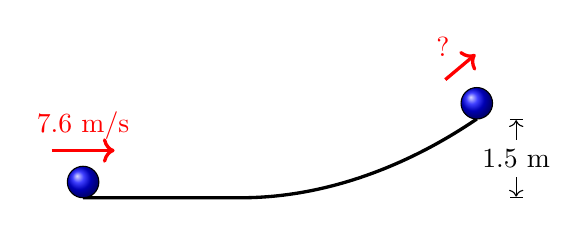
\begin{tikzpicture}
    \draw[very thick] (0,0) -- (2,0) parabola (5,1);
    \draw[shading=ball] (0,.2) circle (.2);
    \draw[red,->,very thick] (-.4,.6) 
      -- (.4,.6) node[midway, above] {7.6 m/s};
    \draw[|<->|] (5.5,0) -- ++(0,1) 
      node[midway, fill=white] {1.5 m};
    \draw[shading=ball] (5,1.2) circle (.2);
    \draw[red,->,very thick] (4.6,1.5) 
      -- ++(40:.5) node[midway, anchor=south east] {?};

      
  \end{tikzpicture}

  \vs[2]


\question
  A 0.24-kg hockey puck is sitting at rest on the ice.  A player exerts a constant 15.6 N of force over a distance of 0.150 m.

  \begin{parts}
    \part
      How much work does the hockey player do on the puck?
      \vs 

    \part
      What is the final velocity of the puck?
      \vs[2]

  \end{parts}



\pagebreak

\question
  A rollercoaster (m = 1000 kg) starts from rest at the top of a 50 m hill.  The tracks are frictionless.

  \begin{parts}
    \part
      If the hill goes all the way down to the ground, how fast should it be going at that point?
    
      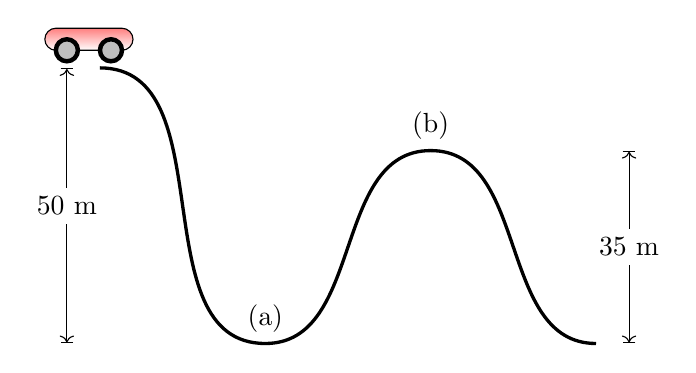
\begin{tikzpicture}[x=0.7cm, y=0.7cm]
        \def\xs{3}
        \draw[very thick] 
          (1*\xs,5) 
          to[in=180,out=0] (2*\xs,0) node[above] {(a)}
          to[in=180,out=0] (3*\xs,3.5) node[above] {(b)}
          to[in=180,out=0] (4*\xs,0);

        \draw[|<->|] (.8*\xs,0) -- (.8*\xs,5) 
          node[midway,fill=white] {50 m};
        \draw[|<->|] (4.2*\xs,0) -- (4.2*\xs,3.5) 
          node[midway,fill=white] {35 m};


        \begin{scope}[scale=0.4,shift={(5,13.3)}]
          \filldraw[top color=red!50, draw=black, rounded corners] 
            (0,0) -- (0,1) -- 
            (4,1) -- (4,0) -- cycle;
          \draw[fill=gray!50, draw=black, ultra thick] 
            (1,0) circle (.5);
          \draw[fill=gray!50, draw=black, ultra thick] 
            (3,0) circle (.5);
        \end{scope}

      \end{tikzpicture}
      \vs

    \part
      Continuing the problem, the rollercoaster continues to the top of the next hill, which is 35 m high.  What is its velocity at the top of the next hill?
      \vs[2]

  \end{parts}


\question
  A 1750-kg car is initially at rest on a flat surface. The driver accelerates the car, covering a distance of 87~meters. The net force acting on the car averages out to 4800~Newtons.  What is the final velocity of the car?
  \vs[2]


  
  
\end{questions}

\end{document}